%%% lorem.tex --- 
%% 
%% Filename: lorem.tex
%% Description: 
%% Author: Ola Leifler
%% Maintainer: 
%% Created: Wed Nov 10 09:59:23 2010 (CET)
%% Version: $Id$
%% Version: 
%% Last-Updated: Tue Oct  4 11:58:17 2016 (+0200)
%%           By: Ola Leifler
%%     Update #: 7
%% URL: 
%% Keywords: 
%% Compatibility: 
%% 
%%%%%%%%%%%%%%%%%%%%%%%%%%%%%%%%%%%%%%%%%%%%%%%%%%%%%%%%%%%%%%%%%%%%%%
%% 
%%% Commentary: 
%% 
%% 
%% 
%%%%%%%%%%%%%%%%%%%%%%%%%%%%%%%%%%%%%%%%%%%%%%%%%%%%%%%%%%%%%%%%%%%%%%
%% 
%%% Change log:
%% 
%% 
%% RCS $Log$
%%%%%%%%%%%%%%%%%%%%%%%%%%%%%%%%%%%%%%%%%%%%%%%%%%%%%%%%%%%%%%%%%%%%%%
%% 
%%% Code:

\chapter{Teori}
\label{cha:theory}

Nedan presenteras hur Entropi estimering, Huffman-kodning och LZW-kodning fungerar.

\subsection{Entropi estimering}
Det går att mäta hur bra komprimerad en sekvens är, detta gör man genom mäta takten på koden. Takten på koden ges av \cite{nautsch2018}.

\bigskip
\noindent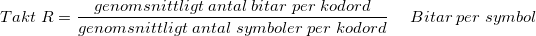
\includegraphics{TaktFormula.png}

\bigskip 
\noindent Det ger alltså ett tal som säger i snitt hur många bitar vi har kodat varje symbol med.

Entropin för en källa är en teoretisk lägre gräns för hur många bitar vi behöver för att koda varje symbol. Takten kan alltså inte vara under denna gräns. Entropin av en källa ges av \cite{nautsch2018}.

\bigskip 
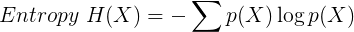
\includegraphics{EntropyFormula.png}

\bigskip 
\noindent Där p(X) är sannolikheten för given symbol och log är logaritm med bas 2. Vi summerar över alla symboler.


\subsection{Huffman-kodning}
Huffman-kodning är en metod för att komprimera filer till ett mindre format. Metoden utvecklades av  den dåvarande studenten David A. Huffman år 1952. Idén med metoden är att tilldela varje symbol som ska kodas med X antal olika bitar, 0 eller 1. Exempel kan symbolen A tilldelas bitarna 101011. I metoden kommer de symboler som förekommer flest gånger i sekvensen, det vill säga den symbol som har högst sannolikhet att förekomma, att tilldelas minst antal bitar. Det betyder också att de symboler som förekommer minst gånger i sekvensen kommer tilldelas mest antal bitar. Exempel kan symbolen A tilldelas med bitarna 10 och symbolen B tilldelas bitarna 1001010101. Detta betyder att symbolen A förekommer oftare i sekvensen än symbolen B. Alltså kommer sekvensen att komprimeras på bästa möjliga vis eftersom A förekommer oftare än B och A:s kodord är kortare än B:s. Redan här inses att med Huffman-kodning behövs information om hur sekvensen ser ut. Det vill säga, man behöver veta sannolikheterna för de olika symbolerna i sekvensen. Nedan beskrivs mer ingående hur komprimering och avkomprimering fungerar i Huffman-kodning \cite{huffmancoding2018}.
	\subsubsection{Komprimering}
	Att komprimera en sekvens med Huffman-kodning förutsätter att det finns en given sannolikhetstabell för sekvensen. Det finns alltså en lista som mappar en symbol mot dess sannolikhet, vi kallar här varje symbol och dess sannolikhet för en nod. Metoden fungerar då enligt följande:
	\begin{enumerate}
	\item Ta ut de två symbolerna (noderna) som har lägst sannolikhet i listan.
	\item Addera dessa noders sannolikheter och lägg till den som en ny nod i listan, resterande noder behålls.
	\item Börja sedan om från ett om det finns fler än en stycken noder kvar i listan.
	\end{enumerate}
	Med den här metoden byggs en trädstruktur upp, som kan ses i figur blablabla, över hur de olika symbolerna kan tilldelas olika bitar. Lövnoderna i trädet representerar de olika symbolerna. Roten av trädet representeras av en nod med sannolikhet 1 eftersom summan av alla sannolikheter i en sekvens alltid summeras till 1. För att tilldela en sekvens av bitar till alla symboler traverserar man igenom hela trädet och bildar en lista som mappar respektive symbol sin egna unika sekvens av bitar. Här är det förutbestämt att varje gång man går vänster i trädet adderar man en 0:a till sekvensen av bitar och varje gång man går höger adderar man en 1:a till sekvensen, eller vice versa. figur blabla visar hur ett Huffman-träd kan se ut \cite{huffmancoding2018}.
	
	När mappningen mellan symbol och sekvens av bitar existerar kan den givna sekvensen komprimeras. Detta görs genom att läsa av en symbol i i taget ifrån sekvensen som ska komprimeras och sedan matcha den symbolen med symbolerna som finns i listan som mappar symboler mot en sekvens av bitar. Då ges en sekvens av bitar som adderas till den resulterande bitsekvensen. Denna procedur upprepas tills det inte finns fler symboler att läsa av i sekvensen som ska komprimeras.  
	\subsubsection{Avkomprimering}
	För att avkomprimera en Huffman-kod behövs samma sannolikhetslista som användes vid komprimeringen av en sekvens. Förutsatt att denna lista är känd, kan ett Huffman-träd byggas upp på samma vis som vid komprimeringen. Med Huffman-trädet kan man sedan traversera ifrån roten och ner beroende på vilken bit, 0 eller 1, man stöter på i den sekvens som ska avkodas. När man sedan kommer till en lövnod betyder det att en symbol kan avkodas, denna symbol adderas sedan till den resulterande sekvensen. Proceduren startar sedan om ifrån rotnoden och avslutas då det inte längre finns bitar kvar att läsa av i bitsekvensen \cite{huffmancoding2018}.
	
\subsection{LZW-kodning}


	\subsubsection{Komprimering}
 
	\subsubsection{Avkomprimering}
	
%%%%%%%%%%%%%%%%%%%%%%%%%%%%%%%%%%%%%%%%%%%%%%%%%%%%%%%%%%%%%%%%%%%%%%
%%% lorem.tex ends here

%%% Local Variables: 
%%% mode: latex
%%% TeX-master: "demothesis"
%%% End: 
